%%%%%%%%%%%%%%%%%%%%%%%%%%%%%%%%%%%%%%%%%%%%%%%%%%%%%%%%%%%%%%%%%%%%%%%%%%%%%%%%
%% MASTER'S THESIS                                                            %%
%%                                                                            %% 
%% Title (en): Multi-Agent Systems and Organizations                          %%
%% Title (cs): Multiagentní systémy a organizace                              %%
%%                                                                            %%
%% Author: Bc. Lukáš Kúdela                                                   %%
%% Supervisor: Prof. RNDr. Petr Štěpánek, DrSc.                               %%
%%                                                                            %%
%% Academic year: 2011/2012                                                   %%
%%%%%%%%%%%%%%%%%%%%%%%%%%%%%%%%%%%%%%%%%%%%%%%%%%%%%%%%%%%%%%%%%%%%%%%%%%%%%%%%

\section{PIM4Agents}

% PIM4Agents - authors
This section introduces the PIM4Agents metamodel\footnote{For ``Platform-independent model for agents''.} \cite{Hahn07a}, \cite{Hahn07b} and \cite{Hahn08} proposed in 2007 by Christian Hahn, Cristián Madrigal-Mora and Klaus Fischer from German Research Centre for Artificial Intelligence (Deutsches Forschungszentrum f\"{u}r K\"{u}nstliche Intelligenz, DFKI).

% Citation
We will present only a brief overview (distilled from \cite{Hahn07b}) since our work does not draw much inspiration from PIM4Agents.

%% PIM4Agents %%%%%%%%%%%%%%%%%%%%%%%%%%%%%%%%%%%%%%%%%%%%%%%%%%%%%%%%%%%%%%%%%%

% PIM4Agents & MDA
PIM4Agents has been specifically designed to be employed in the Model-driven engineering (MDE) software development methodology, more precisely in Model-driven architecture (MDA) by Object Management Group (OMG).
Apart from the platform-independent metamodel itself, the authors have proposed two platform-specific metamodels: JackMM and JadeMM for the JACK and Jade agent platforms respectively.
They have also described two sets of model transformations to convert PIMs to PSMs: PIM4Agents-to-JackMM and PIM4Agents-to-JadeMM.

%%%%%%%%%%%%%%%%%%%%%%%%%%%%%%%%%%%%%%%%%%%%%%%%%%%%%%%%%%%%%%%%%%%%%%%%%%%%%%%%
\subsection*{Core Model}

% Core metamodel
To support adaptability, PIM4Agents is structured around a small core that could be augmented with extensions to model specific aspects of MASs, for example, security.
Figure~\ref{figure:pim4agents-metamodel} shows the core model.

% Agent
The metamodel, like previously introduced metamodels, is built around the concept of \textit{Agent}, an autonomous entity capable of sensing its environment and acting upon it.
Each \textit{Agent} has access to a set of \textit{Resources} from its surrounding \textit{Environment} \cite{Hahn07b}.

% Behaviour, Capability
A \textit{Behaviour} can be atomic or composed of sub-behaviours.
This way, a whole hierarchy of specific \textit{Behaviours} can be created.
A \textit{Behaviour} may also send or receive \textit{Messages} according to a \textit{Protocol}.
A \textit{Capability} allows to group conceptually related \textit{Behaviours} \cite{Hahn07b}.

% Role, Cooperation, Protocol, Message
A \textit{Role} is an abstraction of the social behaviour of an \textit{Agent} in a given social context, usually a \textit{Cooperation}; it specifies the responsibilities of a \textit{Agent} in that social context.
A \textit{Cooperation} represents the interaction between \textsc{Agents} playing the required set of \textit{Roles}.
The detailed realisation of this interaction is described by a \textit{Protocol} that specifies the \textit{Messages} exchanged between the \textit{Roles} and at which point in time they are to be expected.
A \textit{Protocol} is executed by a set of \textit{Behaviours} sending and receiving \textit{Messages} in accordance to their \textit{Roles}.

% Organziation
\textit{Agents} can take part in an \textit{Organization}, a special kind of \textit{Cooperation} that also has the same characteristics as an \textit{Agent}.
Being a \textit{Cooperation}, an \textit{Organization} can have its own internal protocol that specifies how it coordinates its members.
Being also an \textit{Agent}, an \textit{Organization} can play roles in other \textit{Organizations} (super-organization) and has \textit{Capabilities} which can be performed by its members, be they \textit{Agents} or other \textit{Organizations} (sub-organizations).

% Figure: PIM4Agents metamodel
\begin{figure}[ht]
	\centering
	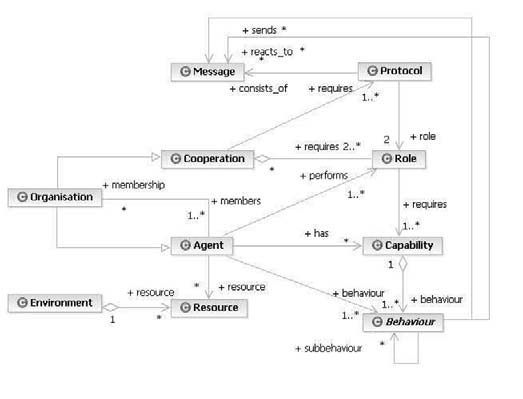
\includegraphics[width=0.6\textwidth]{images/pim4agents/pim4agents-metamodel.png}
	\caption{The PIM4Agents core model \cite{Hahn07b}}
	\label{figure:pim4agents-metamodel}
\end{figure}

%%%%%%%%%%%%%%%%%%%%%%%%%%%%%%%%%%%%%%%%%%%%%%%%%%%%%%%%%%%%%%%%%%%%%%%%%%%%%%%%
\subsection{JadeOrgs}

JadeOrgs
\cite{Madrigal-Mora08} and \cite{Madrigal-Mora09}
is an extension of the Jade framework that implements the JadeMM platform-specific metamodel.

JadeMM is defined using Eclipse Modeling Framework (EMF) to exploit EMF's code generation facility.
Given a platform-independent model of a MAS (conforming to PIM4Agents), the corresponding Jade/JadeOrgs platform-specific model (conforming to JadeMM) can be derived automatically.